\section{Introducción}

\textbf{La productividad laboral no solo varía entre actividades económicas, sino también entre territorios.} El Informe 01 de esta serie mostró que el crecimiento de la productividad en Colombia es muy heterogéneo entre ramas de actividad económica. Este segundo informe replica la misma lógica de medición, pero ahora a nivel departamental. La pregunta central es sencilla: ¿en qué departamentos creció más la producción por trabajador y por hora trabajada?

\textbf{La mirada territorial es importante porque la productividad refleja condiciones locales de estructura productiva, infraestructura, capital humano, informalidad, conectividad y capacidad institucional.} Dos departamentos pueden tener el mismo crecimiento de ocupados y, sin embargo, trayectorias muy distintas de productividad si difieren en la composición de sus actividades, en la calidad del empleo o en la capacidad de absorber inversión y tecnología.

\textbf{El objetivo de este informe es medir la evolución de la productividad laboral departamental en Colombia entre 2014 y 2024pr.} Para ello se combina el Producto Interno Bruto por regiones del DANE, expresado en pesos constantes de 2015, con ocupados y horas trabajadas de la Gran Encuesta Integrada de Hogares (GEIH). Bogotá se trata como si fuera un departamento para mantener una unidad territorial comparable con el anexo departamental de cuentas nacionales.

\textbf{El informe está organizado en cinco secciones, incluyendo esta introducción.} La sección 2 presenta la metodología y las fuentes. La sección 3 compara la productividad laboral de los departamentos. La sección 4 analiza la relación entre crecimiento del trabajo y crecimiento de la productividad. La sección 5 presenta conclusiones. El apéndice incluye el detalle de cada departamento.

\section{Metodología}

\textbf{La medición combina cuentas nacionales departamentales y microdatos de la GEIH.} El numerador corresponde al PIB departamental real del DANE, tomado del anexo \textit{Producto Interno Bruto por regiones}, en series encadenadas de volumen con año de referencia 2015. El denominador se construye con la GEIH, sumando ocupados con el factor de expansión \texttt{fex} y calculando horas anuales como horas semanales ponderadas multiplicadas por 52.

\textbf{Se construyen dos indicadores de productividad laboral.} El PIB por trabajador divide el PIB real departamental entre el número anual de ocupados del departamento. El PIB por hora trabajada divide el mismo PIB entre el total anual de horas trabajadas. La segunda medida corrige por cambios en la intensidad horaria y, por tanto, permite distinguir si un aumento del producto por trabajador proviene de producir más por hora o de trabajar más horas.

\textbf{El periodo de análisis es 2014--2024pr.} Esta ventana corresponde a la serie disponible en el anexo departamental del DANE. Se excluye 2020 para mantener consistencia con el tratamiento del Informe 01, dado que la base anual de GEIH usada en el proyecto no considera ese año como comparable. Las tasas de crecimiento reportadas son tasas anualizadas entre 2014 y 2024.

\section{Productividad laboral por departamento}

\textbf{La productividad laboral departamental presenta una dispersión amplia.} El Cuadro \ref{tab:pib_geih_productividad_departamento} ordena los departamentos por crecimiento del PIB por hora trabajada entre 2014 y 2024pr. La lectura conjunta del PIB por trabajador y el PIB por hora es útil porque algunos departamentos pueden mostrar mejoras por trabajador aun cuando parte de esa mejora provenga de cambios en las horas trabajadas.

\begin{table}[H]
\centering
\caption{Productividad laboral por departamento, 2014--2024pr}
\label{tab:pib_geih_productividad_departamento}
\scriptsize
\begin{tabular}{lrrrr}
\toprule
Departamento & PIB/trab. 2024 & PIB/hora 2024 & Crec. PIB/trab. & Crec. PIB/hora \\
\midrule
Quindío & 33,8 & 15,1 & 7,21\% & 8,21\% \\
Putumayo & 443,0 & 202,1 & 6,27\% & 6,62\% \\
Risaralda & 38,7 & 16,4 & 3,37\% & 4,14\% \\
Caquetá & 24,9 & 10,5 & 3,51\% & 3,88\% \\
Caldas & 36,6 & 15,6 & 2,36\% & 2,81\% \\
Sucre & 22,0 & 10,4 & 2,03\% & 2,79\% \\
San Andrés y Providencia & 82,4 & 33,3 & 2,86\% & 2,78\% \\
Bogotá D.C. & 67,4 & 28,6 & 2,05\% & 2,44\% \\
Boyacá & 47,5 & 22,6 & 1,49\% & 2,16\% \\
Tolima & 40,0 & 16,9 & 1,76\% & 1,75\% \\
Valle del Cauca & 54,5 & 23,5 & 1,39\% & 1,72\% \\
Santander & 62,0 & 26,1 & 1,40\% & 1,68\% \\
Chocó & 28,6 & 11,9 & 1,96\% & 0,89\% \\
Bolívar & 45,1 & 19,8 & 0,61\% & 0,82\% \\
Norte de Santander & 24,3 & 10,0 & 0,94\% & 0,79\% \\
Vichada & 92,2 & 38,1 & 1,33\% & 0,77\% \\
Nariño & 17,8 & 9,1 & -0,49\% & 0,46\% \\
Cauca & 26,6 & 13,7 & -0,21\% & 0,32\% \\
Córdoba & 22,0 & 10,7 & 0,16\% & 0,25\% \\
Antioquia & 47,7 & 20,3 & -0,09\% & 0,21\% \\
Amazonas & 50,2 & 21,8 & -0,09\% & 0,20\% \\
Magdalena & 23,9 & 10,3 & 0,00\% & 0,17\% \\
Guaviare & 39,1 & 17,0 & -1,00\% & -0,14\% \\
La Guajira & 24,8 & 11,1 & -0,71\% & -0,39\% \\
Arauca & 171,2 & 66,8 & -0,28\% & -0,84\% \\
Huila & 31,6 & 14,2 & -1,31\% & -0,86\% \\
Cesar & 32,6 & 13,8 & -1,61\% & -1,07\% \\
Guainía & 38,8 & 17,0 & -1,46\% & -1,23\% \\
Atlántico & 37,3 & 16,0 & -1,77\% & -1,33\% \\
Cundinamarca & 40,4 & 17,4 & -1,69\% & -1,53\% \\
Meta & 63,1 & 25,9 & -2,67\% & -2,07\% \\
Vaupés & 58,5 & 26,2 & -3,31\% & -2,75\% \\
Casanare & 165,2 & 67,8 & -3,31\% & -3,33\% \\
\bottomrule
\end{tabular}
\caption*{\footnotesize Nota: PIB por trabajador en millones de pesos constantes de 2015; PIB por hora en miles de pesos constantes de 2015. Bogotá se trata como departamento. Se excluye 2020 por no contar con GEIH anual comparable en la base del proyecto. Fuente: cálculos propios con DANE, Cuentas Nacionales Departamentales, y GEIH.}
\end{table}

\textbf{Los departamentos con mayor crecimiento del PIB por hora trabajada fueron Quindío, Putumayo y Risaralda.} En Quindío, el PIB por hora creció 8,21\% anual y el PIB por trabajador 7,21\% anual. En Putumayo, el PIB por hora creció 6,62\% anual y el PIB por trabajador 6,27\% anual. Estos casos combinan aumentos de productividad con reducciones de ocupados, lo que sugiere que parte del resultado puede reflejar cambios en la composición o escala del empleo departamental.

\textbf{En el otro extremo se ubican Casanare, Vaupés y Meta.} Casanare registra una caída anual de 3,33\% en el PIB por hora y de 3,31\% en el PIB por trabajador. Vaupés y Meta también muestran caídas importantes de productividad, a pesar de aumentos en la ocupación. En estos casos, el aumento del trabajo no estuvo acompañado por un aumento proporcional del PIB real departamental.

\begin{figure}[H]
  \centering
  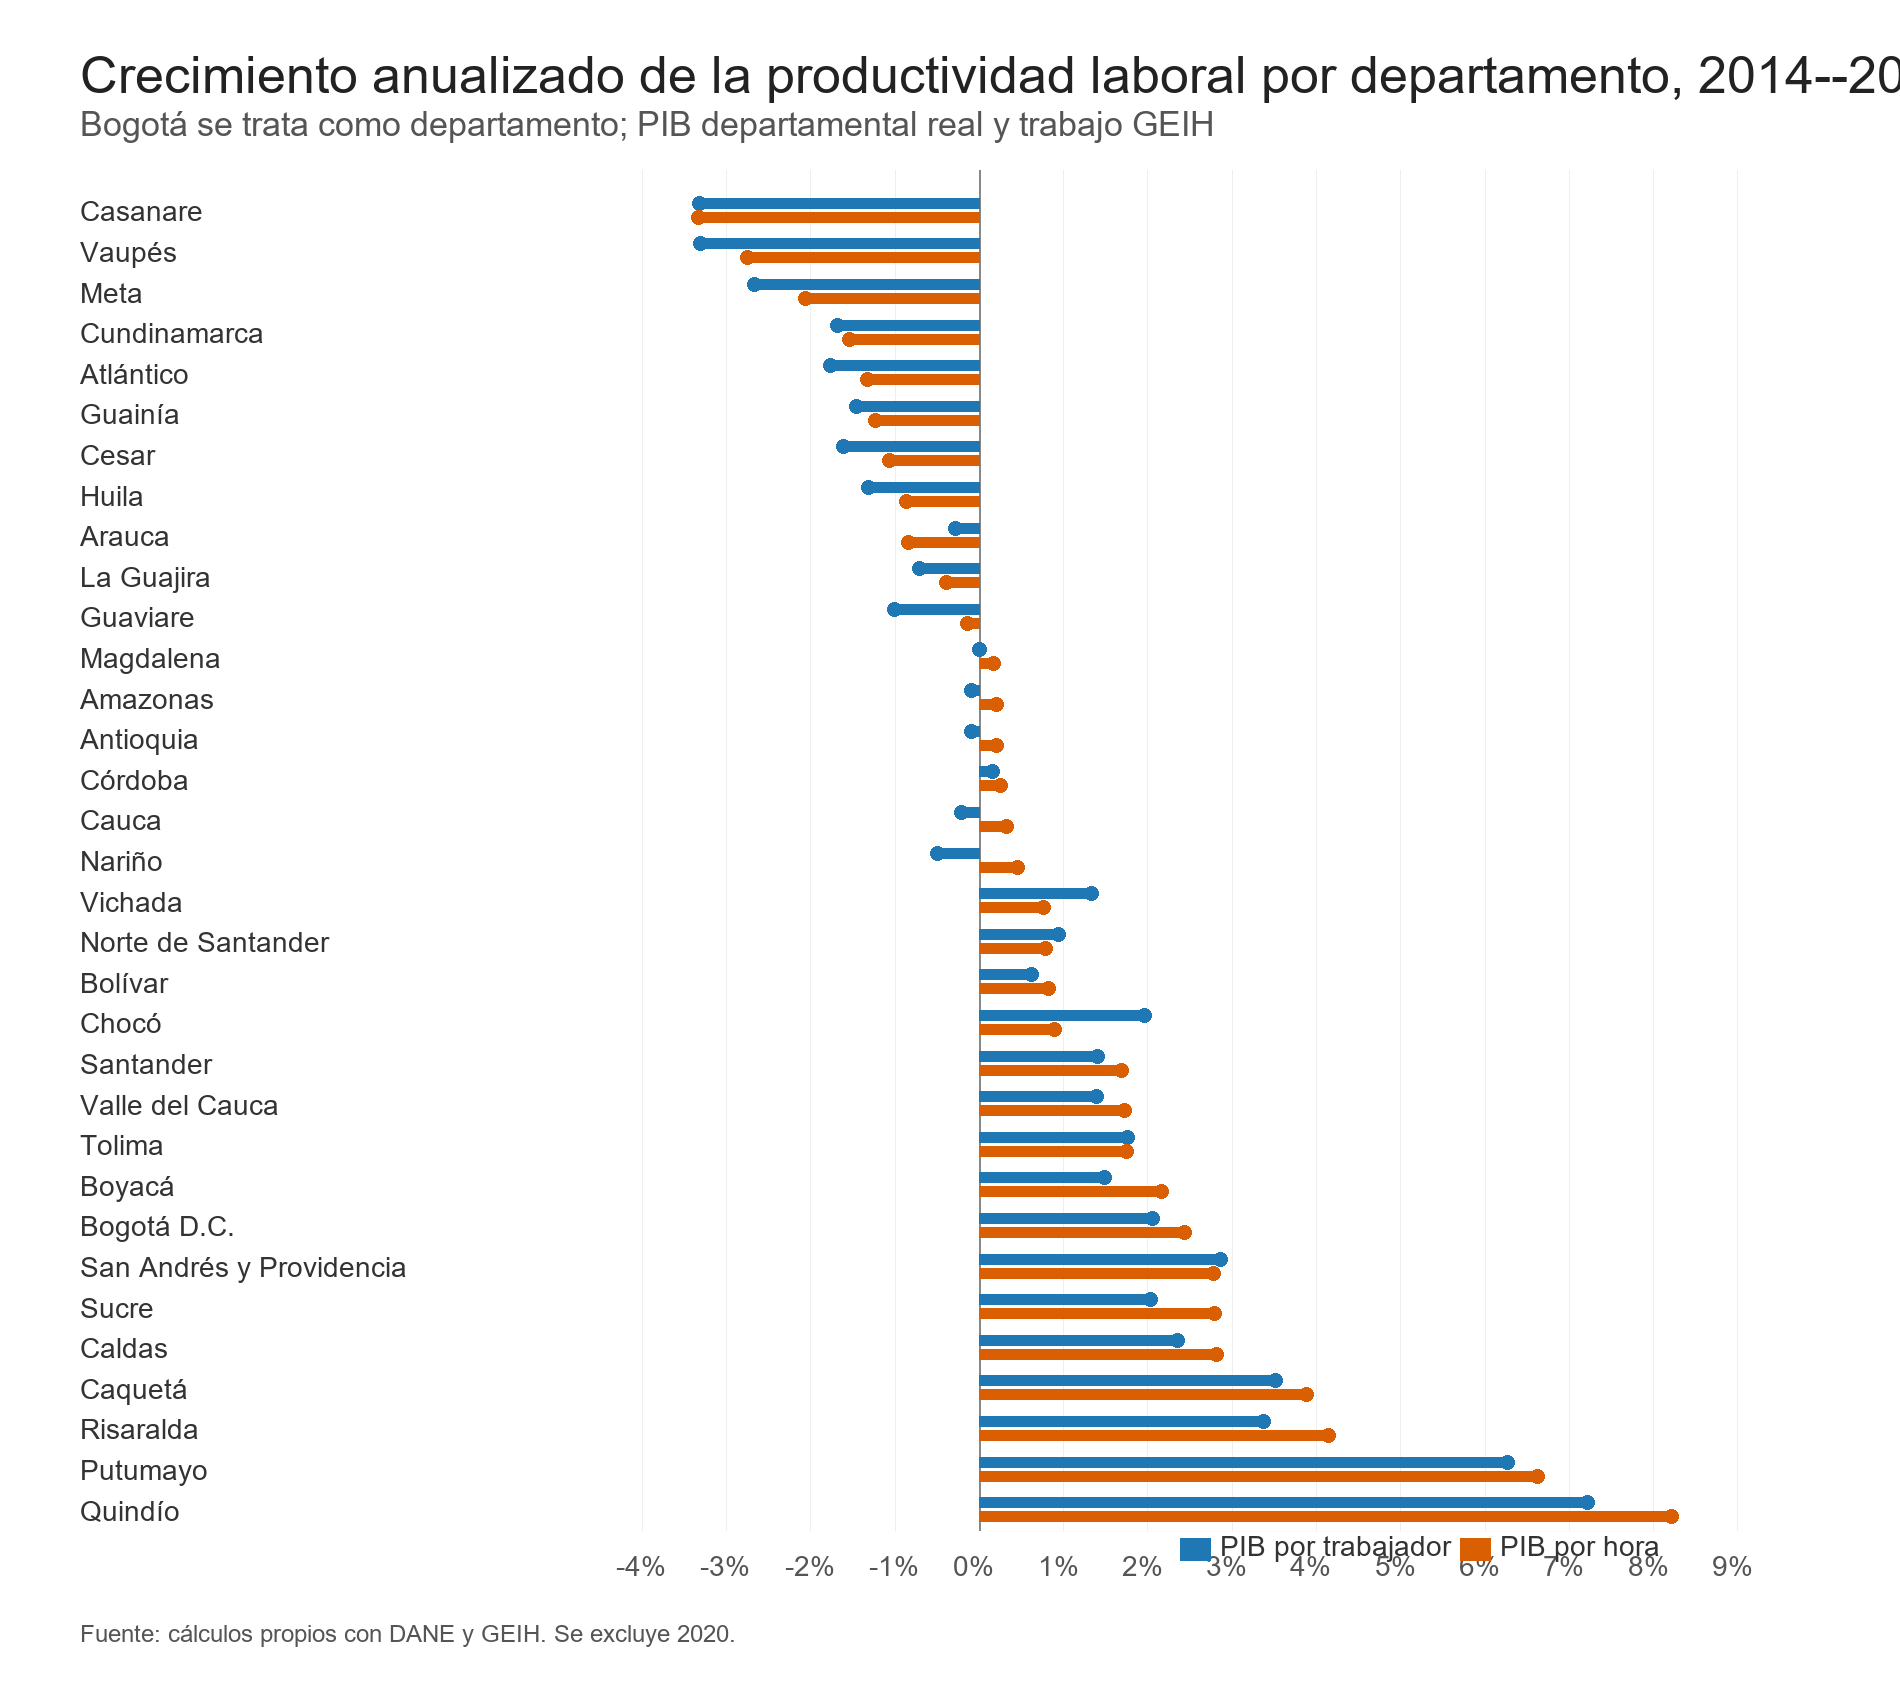
\includegraphics[width=\textwidth]{Paper/figures/fig_pib_geih_productividad_departamento.png}
  \caption{Crecimiento anualizado de la productividad laboral por departamento, 2014--2024pr}
  \label{fig:pib_geih_productividad_departamento}
\end{figure}

\textbf{La Figura \ref{fig:pib_geih_productividad_departamento} permite ver que las diferencias no son marginales.} La distancia entre los departamentos de mayor y menor crecimiento supera diez puntos porcentuales anuales cuando se mide la productividad por hora. Esto confirma que el desempeño agregado del país oculta trayectorias territoriales muy diferentes.

\section{Crecimiento del trabajo y crecimiento de la productividad}

\textbf{Una pregunta natural es si la ocupación creció más en los departamentos donde también creció más la productividad.} Esta relación importa porque el crecimiento económico se acelera cuando el trabajo se expande en territorios donde la producción por trabajador o por hora también aumenta. En cambio, si el empleo crece en territorios con productividad estancada o decreciente, el aumento del producto puede depender más de absorber trabajo que de producir más eficientemente.

\begin{table}[H]
\centering
\caption{Correlaciones departamentales entre crecimiento del trabajo y crecimiento de la productividad}
\label{tab:pib_geih_productividad_departamento_correlaciones}
\begin{tabular}{llr}
\toprule
Variable 1 & Variable 2 & Correlación \\
\midrule
Crec. ocupados & Crec. PIB por trabajador & -0,91 \\
Crec. ocupados & Crec. PIB por hora & -0,89 \\
Crec. horas totales & Crec. PIB por trabajador & -0,91 \\
Crec. horas totales & Crec. PIB por hora & -0,92 \\
PIB por hora inicial & Crec. PIB por hora & -0,08 \\
\bottomrule
\end{tabular}
\caption*{\footnotesize Nota: correlaciones de Pearson calculadas entre departamentos, tratando a Bogotá como departamento. Fuente: cálculos propios con DANE y GEIH.}
\end{table}

\begin{figure}[H]
  \centering
  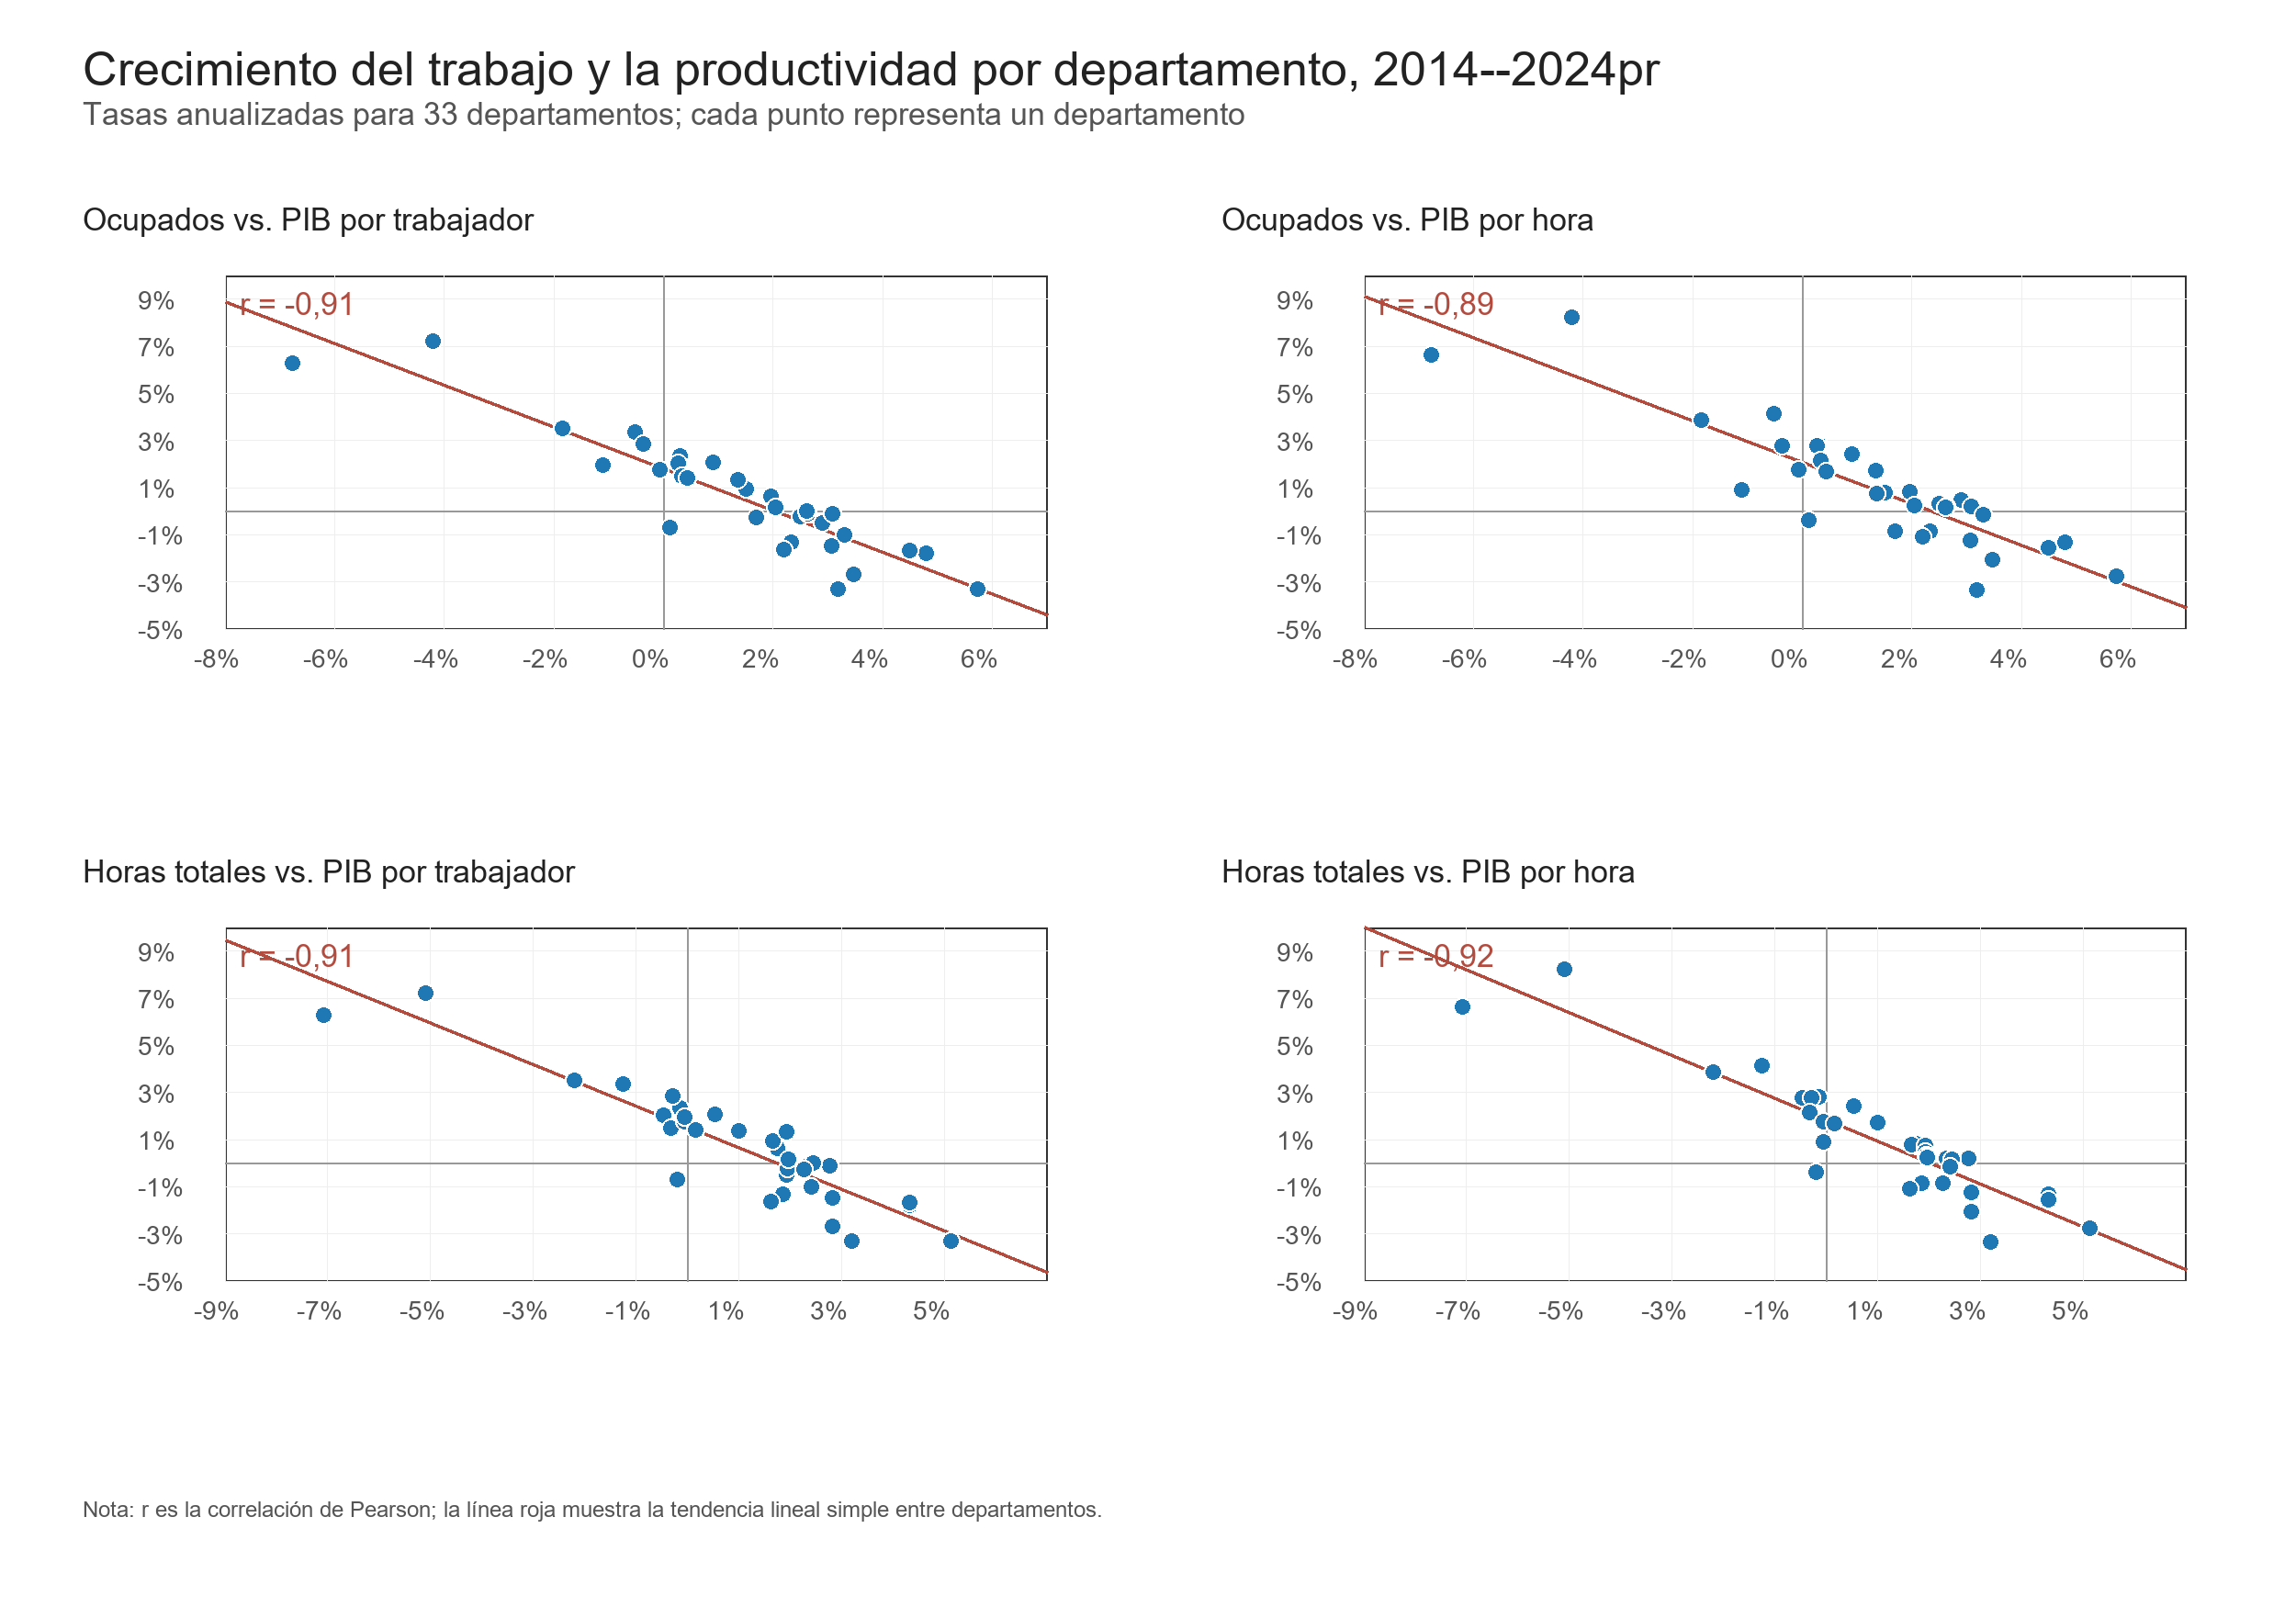
\includegraphics[width=\textwidth]{Paper/figures/fig_pib_geih_productividad_departamento_correlaciones.png}
  \caption{Crecimiento del trabajo y crecimiento de la productividad por departamento}
  \label{fig:pib_geih_productividad_departamento_correlaciones}
\end{figure}

\textbf{Los resultados sugieren que el crecimiento del trabajo y el crecimiento de la productividad no avanzaron de la mano.} Algunos departamentos con alto crecimiento de ocupados, como Vaupés, Atlántico y Cundinamarca, registran caídas del PIB por hora trabajada. En contraste, Quindío y Putumayo combinan alto crecimiento de productividad con caídas de ocupación. Esta relación negativa debe interpretarse con cautela, pues puede reflejar migración, cambios en composición sectorial, variaciones de precios relativos reales encadenados o choques específicos de actividades dominantes en cada territorio.

\textbf{La comparación territorial no reemplaza el análisis sectorial: lo complementa.} Un departamento con caída de productividad puede estar afectado por una actividad específica con bajo desempeño, mientras que otro puede mejorar porque cambia la composición de su empleo hacia actividades de mayor valor agregado. Por eso, la siguiente etapa natural del proyecto es cruzar simultáneamente actividad económica y departamento, siempre que las fuentes permitan una medición laboral suficientemente confiable.

\section{Conclusiones}

\textbf{El análisis departamental muestra que la productividad laboral colombiana tiene una dimensión territorial fuerte.} La diferencia entre departamentos líderes y rezagados es grande tanto en niveles como en crecimiento. Esto implica que la agenda de productividad no puede limitarse a una mirada nacional promedio.

\textbf{La productividad por hora ofrece una lectura más precisa que la productividad por trabajador cuando las horas trabajadas cambian.} En varios departamentos, el crecimiento del PIB por trabajador y el crecimiento del PIB por hora no son idénticos porque las horas semanales por trabajador se movieron durante el periodo. La distinción es relevante para evaluar si la mejora de productividad implica producir más eficientemente o simplemente trabajar más.

\textbf{El crecimiento de ocupados no siempre se concentró en los departamentos con mayor crecimiento de productividad.} Esta evidencia no prueba por sí sola una mala asignación territorial del trabajo, pero sí señala una pregunta importante para la política pública: qué condiciones permiten que el crecimiento del empleo ocurra junto con aumentos sostenidos de producción por hora.

\textbf{Una agenda territorial de productividad debe identificar los mecanismos detrás de estas diferencias.} Entre los candidatos están la composición sectorial, la infraestructura, la calidad del empleo, la informalidad, la educación, la inversión privada y la capacidad de los territorios para conectar empresas y trabajadores con mercados más amplios. Este informe ofrece una primera medición descriptiva para orientar ese diagnóstico.
